\documentclass[a4paper,12pt]{article}
\usepackage[utf8x]{inputenc} %fac
%\usepackage[utf8]{inputenc} %fac

\usepackage[sectionbib]{natbib}
%\usepackage{chapterbib}

\usepackage[francais]{babel} %FR
\usepackage[T1]{fontenc}
\usepackage{fancyhdr}

\usepackage[pdftex]{graphicx} % img
%\usepackage{wrapfig} %fac
\usepackage{float}

% \usepackage{embedfile} %inclure fichier

%\usepackage{algpseudocode} %fac
\usepackage[hidelinks=true]{hyperref} %fac

\usepackage[top=3.5cm, bottom=3.5cm, left=3cm, right=3cm]{geometry} %Réduire les marges

% \usepackage{showkeys}
% \usepackage{showlabels}
\usepackage{nameref}

% Style Page
\pagestyle{fancy} % entêtes

\setlength{\headheight}{15pt}
\lhead{ \leftmark }
\rhead{ %\rightmark 
}

%\usepackage{lscape} %une page en portrait

\sloppy % ne pas faire déborder les lignes dans la marge

%\setcounter{tocdepth}{1} %hideallsubsections

\renewcommand{\bibsection}{\subsection{Références}} %Références as subsection


\begin{document}
  \begin{titlepage}
   \def\titletype{Plan de développement}
   %%%%%%%%%%%%%%%%%%%%%%%%%%%%%%%%%%%%%%%%%
% University Assignment Title Page
% LaTeX Template
%
% This template has been downloaded from:
% http://www.latextemplates.com
%
% Original author:
% WikiBooks (http://en.wikibooks.org/wiki/LaTeX/Title_Creation)
%
% Instructions for using this template:
% This title page is presently capable of being compiled as is. This is not
% useful for including it in another document. To do this, you have two options:
%
% 1) Copy/paste everything between \begin{document} and \end{document}
% starting at \begin{titlepage} and paste this into another LaTeX file where you
% want your title page.
% OR
% 2) Remove everything outside the \begin{titlepage} and \end{titlepage} and
% move this file to the same directory as the LaTeX file you wish to add it to.
% Then add \input{./title_page_1.tex} to your LaTeX file where you want your
% title page.
%
%%%%%%%%%%%%%%%%%%%%%%%%%%%%%%%%%%%%%%%%%

%----------------------------------------------------------------------------------------
%       PACKAGES AND OTHER DOCUMENT CONFIGURATIONS
%----------------------------------------------------------------------------------------

\begin{titlepage}

\newcommand{\HRule}{\rule{\linewidth}{0.5mm}} % Defines a new command for the horizontal lines, change thickness here

\center % Center everything on the page

%----------------------------------------------------------------------------------------
%       HEADING SECTIONS
%----------------------------------------------------------------------------------------

\textsc{\LARGE Pierre and Marie Curie University}\\[1.5cm] % Name of your university/college
\textsc{\Large \titletype}\\[0.5cm] % Major heading such as course name
%\textsc{\large PIAD de Master1 d’Informatique en Intelligence Artificielle et Décision}\\[0.5cm] % Minor heading such as course title

%----------------------------------------------------------------------------------------
%       TITLE SECTION
%----------------------------------------------------------------------------------------

\HRule \\[0.4cm]
{ \huge \bfseries \majortitle}\\[0.4cm] % Title of your document
\HRule \\[1.5cm]


%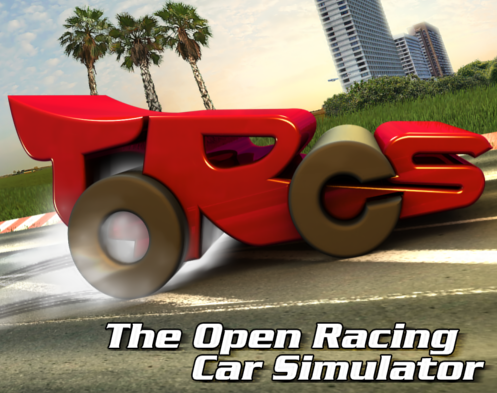
\includegraphics[height=60mm]{images/torcs.png}\\[1cm]


%----------------------------------------------------------------------------------------
%       AUTHOR SECTION
%----------------------------------------------------------------------------------------

\begin{minipage}{0.4\textwidth}
\begin{flushleft} \large
\emph{Author:}\\
Matthieu \textsc{Zimmer} % Your name
\end{flushleft}
\end{minipage}
~
\begin{minipage}{0.4\textwidth}
\begin{flushright} \large
\emph{Supervisors:} \\
Paolo \textsc{Viappiani}\\ % Supervisor's Name
Paul \textsc{Weng}\\ % Supervisor's Name
\end{flushright}
\end{minipage}\\[1cm]

\vfill

%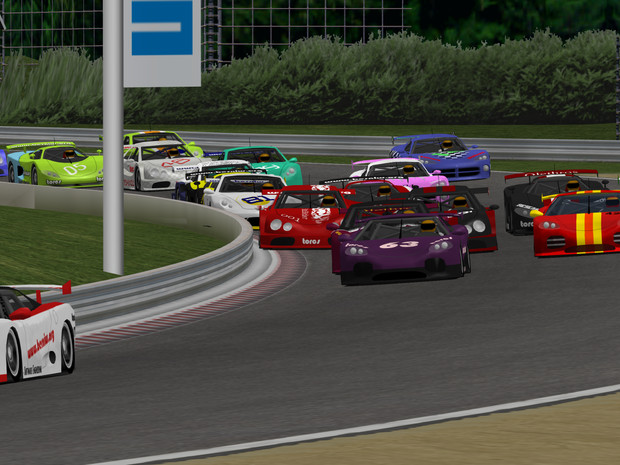
\includegraphics[height=70mm]{images/torcs.jpg}\\[1cm]

%----------------------------------------------------------------------------------------
%       DATE SECTION
%----------------------------------------------------------------------------------------

{\large \today}\\[3mm] % Date, change the \today to a set date if you want to be precise
{\large Version \docversion}\\[1.5cm]

%----------------------------------------------------------------------------------------
%       LOGO SECTION
%----------------------------------------------------------------------------------------


\includegraphics[height=13mm]{../images/logo.png} % Include a department/university logo - this will require the graphicx package

%----------------------------------------------------------------------------------------

% \vfill % Fill the rest of the page with whitespace

\end{titlepage}

  \end{titlepage}

  
  \clearpage

  \tableofcontents

  \clearpage
  
  \renewcommand{\labelitemi}{$\bullet$}
  \renewcommand{\labelitemii}{$\circ$}
  \renewcommand{\labelitemiii}{$\diamond$}
  \renewcommand{\labelitemiv}{$\ast$}
  
  \section{Apercu du TER} 

  \subsection{Objectifs}
	Nous devrons développer une bibliothèque indépendante du domaine dans lequel l'agent évolue. 
	Elle fournira plusieurs algorithmes de base de l'apprentissage par renforcement  (Q-Learning, SARSA, …), 
	plusieurs critères de performance, ainsi qu'une ouverture sur l'apprentissage semi-supervisé : 
	c'est à dire avec les retours de l'expert pris en compte. 
	
	Dans un premier temps, l'expert pourra simplement compenser la fonction de récompense en précisant si 
	l'agent a bien ou mal agit. Dans un second temps, si le temps le permet, l'expert pourra également agir 
	sur le choix de l'action à entreprendre lors de l'exploration de l'agent, ou encore dire à l'agent s'il 
	est temps d'exploiter ou d'explorer.
	
	Parallèlement au développement de la bibliothèque, afin d'avoir une application pratique de la théorie,
	on utilisera ces algorithmes dans le simulateur TORCS sur l'apprentissage automatique de la conduite de 
	voiture sur circuit. Nous modifierons également l'interface TORCS pour intégrer les retours positifs ou 
	négatif de l'expert, voire des retours plus complexes cité précédemment. \cite{CdC}

  
  \nocite{TORCS}
  
  \bibliographystyle{../dependance/apalike}
  \bibliography{../dependance/biblio}

     
  %\vfill

  \subsection{Définitions et acronymes} 
  
  \paragraph{Env. Réduit} Il s'agit de l'environnement de TORCS avec des perceptions limitées pour l'agent conducteur :
    \begin{itemize}
     \item son angle (par rapport à la droite au milieu de la route)
     \item la distance entre son centre de gravité et le milieu de la route
     \end{itemize}
     ainsi que des actions limitées pour la voiture :
    \begin{itemize}
    \item son accélérateur
    \item son freinage
    \item sa direction
    \end{itemize}
    On s'attend donc à ce que l'agent dans cette environnement roule toujours avec la première vitesse.
  
  \paragraph{Env. Complexe}Il s'agit toujours de l'environnement de TORCS mais agrémenté de nouvelles perceptions
    \begin{itemize}
     \item coincé ou non (dans un mur)
     \item vitesse (pour savoir comment accélérer/freiner)
     \item RPM (pour savoir quelle vitesse mettre)
     \item friction du sol (pour déterminer s'il est sur la route ou en dehors, quel type de terrain, ...)
     \item distance du prochain virage (pour déterminer l'accélération et la vitesse maximale)
     \item angle du prochain virage (pour le prendre plus sec)
    \end{itemize}
    et de nouvelles actions
    \begin{itemize}
     \item boîte à vitesse
    \end{itemize}
    
   \paragraph{CdC} Cahier des charges
   
   \paragraph{PdP} Plan de développement
   
   \paragraph{APR} Apprentissage par Renforcement
   
  \bigskip
  En plus de ces définitions, les documents permettant de bien 
    comprendre le plan sont les suivants : \cite{PDMIA} et \cite{ReinforceLearningIntro}.
  
  \newpage 
  \section{Organisation du TER}

    \subsection{Participants}
	Encadrants :
	\begin{itemize}
		\item Paolo \textsc{Viappiani} (\href{mailto:Paolo.Viappiani@lip6.fr}{Paolo.Viappiani@lip6.fr})
		\item Paul \textsc{Weng} (\href{mailto:Paul.Weng@lip6.fr }{Paul.Weng@lip6.fr})
	\end{itemize}

	\bigskip
	Etudiants :
	\begin{itemize}
		\item Lan \textsc{Zhou} (\href{mailto:lan\_612zhou@yahoo.cn}{lan\_612zhou@yahoo.cn})
		\item Matthieu \textsc{Zimmer} (\href{mailto:contact@matthieu-zimmer.net}{contact@matthieu-zimmer.net})
	\end{itemize}

	\bigskip
	À l'heure actuelle, il n'y a pas de liens avec d'autres TER, enseignants, chercheurs,
	laboratoires, entreprises.
    
    \subsection{Activités globales}
      \paragraph{Scripts} Maintenir et développer un ensemble de script permettant de compiler, installer, nettoyer, lancer
      des tests et faciliter l'ensemble du developpement du projet.
      
      \paragraph{Documentation} Gérer et 
      
      \paragraph{Intégration Linux} Maintenir la compatibilité des sources sous le système Linux.
      
      \paragraph{Intégration Mac} Maintenir la compatibilité des sources sous le système Mac.

    \subsection{Tâches jalonnées}
    
      \paragraph{Conception bibliothèque} Réfléchir aux différentes classes et méthodes nécessaire pour concevoir une
      bibliothèque réutilisable. Concevoir les diagrammes de classe.
      
      \paragraph{Implémentation Q-learning} Implémenter l'algorithme Q-learning dans la bibliothèque de façon générique
      et réutilisable.
      
      \paragraph{Implémentation SARSA}  Implémenter l'algorithme SARSA dans la bibliothèque de façon générique
      et réutilisable.
      
      \paragraph{Interfacer Q-learning - Env. Réduit}
      
      \paragraph{Interfacer SARSA - Env. Réduit}
      
      \paragraph{Implémentation fonction d'approximation}
      
      \paragraph{Interfacer Q-learning - Env. Complexe}
      
      \paragraph{Interfacer SARSA - Env. Complexe}
      
      \paragraph{Implémenter mesure de Perf.}
      
      \paragraph{Implémenter fonction de Récompenses}
      
      \paragraph{Modifier interface TORCS}
    
    \subsection{Rôles et responsabilités} test
	    
    \subsection{Calendrier} 
      \begin{figure}[h!]
	\centerline{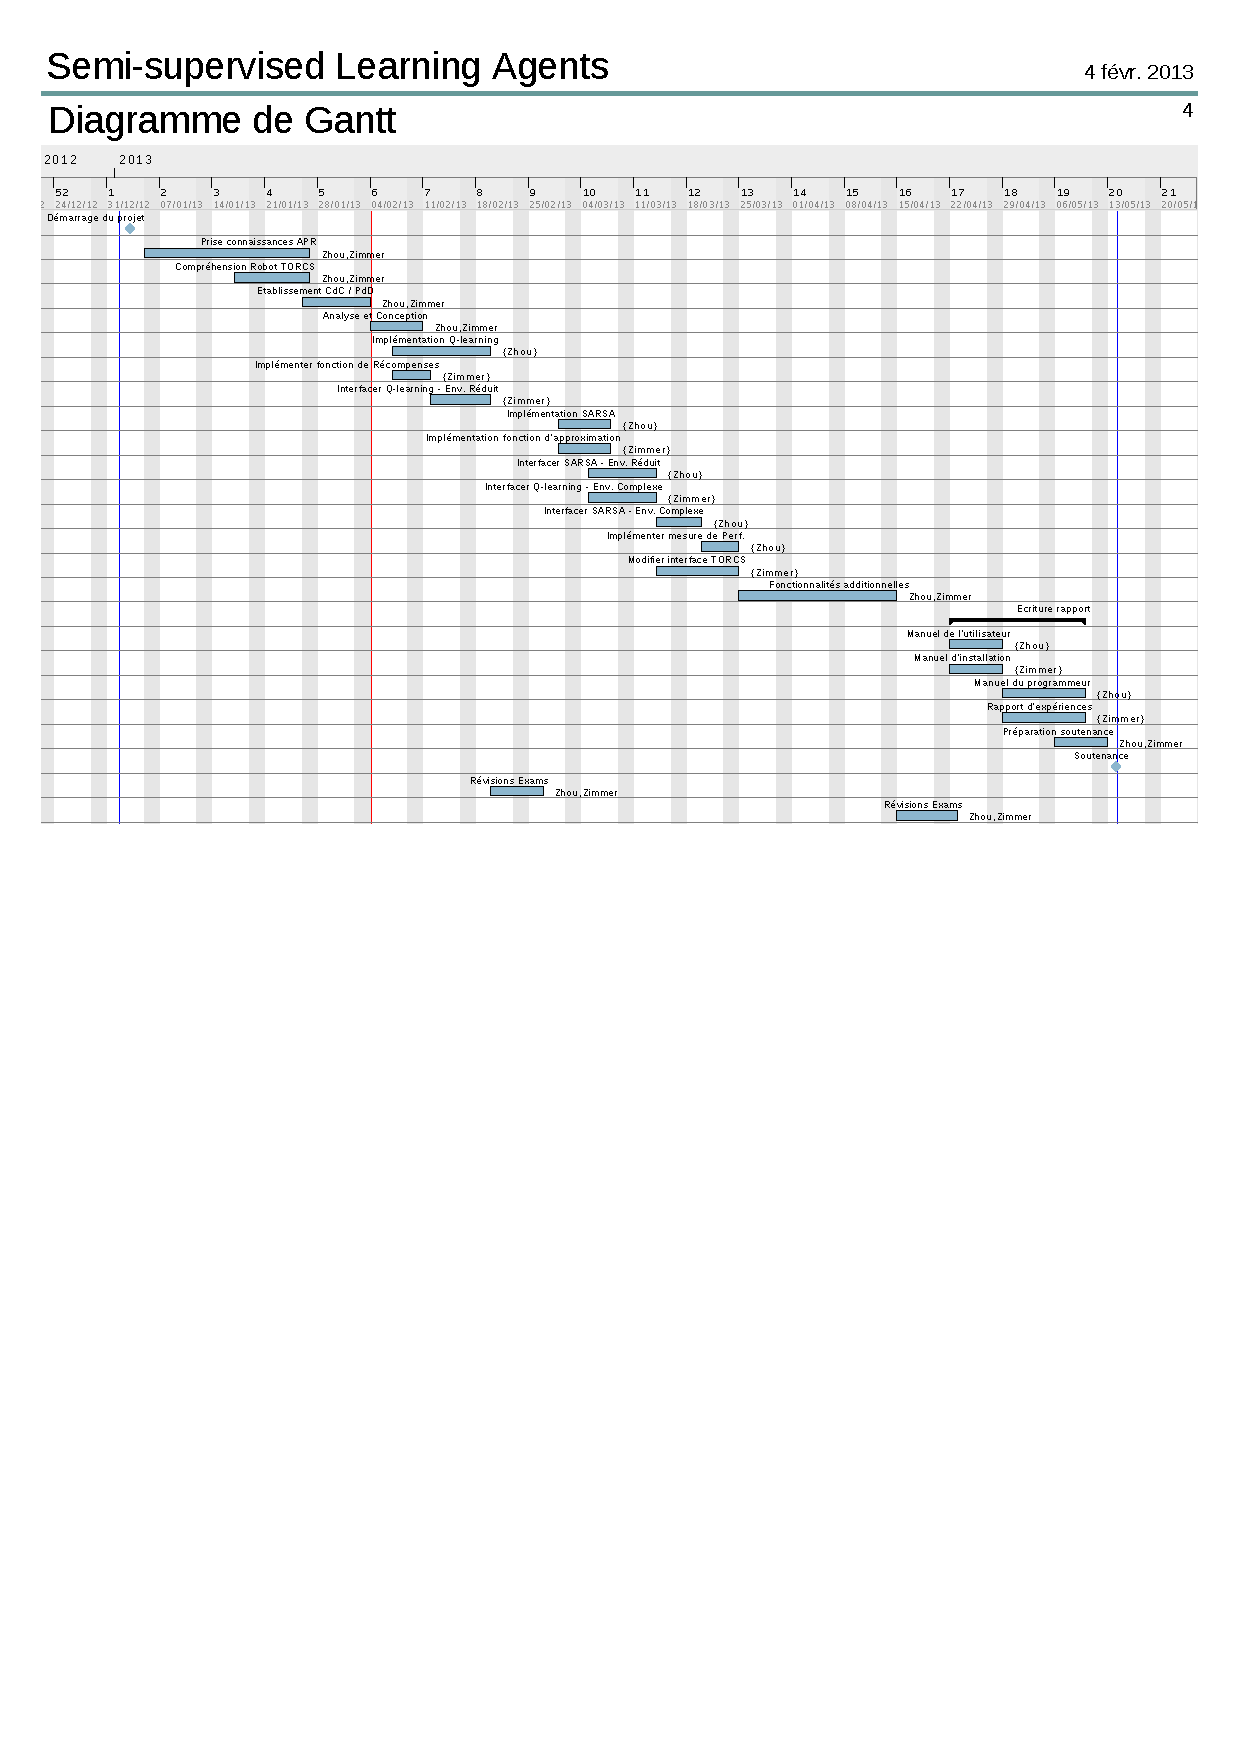
\includegraphics[width=20cm, clip=true, trim= 0 450 0 72]{../images/Gantt.pdf} }
	\caption{Diagramme de Gantt \scriptsize{(zoomer pour meilleur qualité)}}
      \end{figure}

      \begin{figure}[h!]
	\centerline{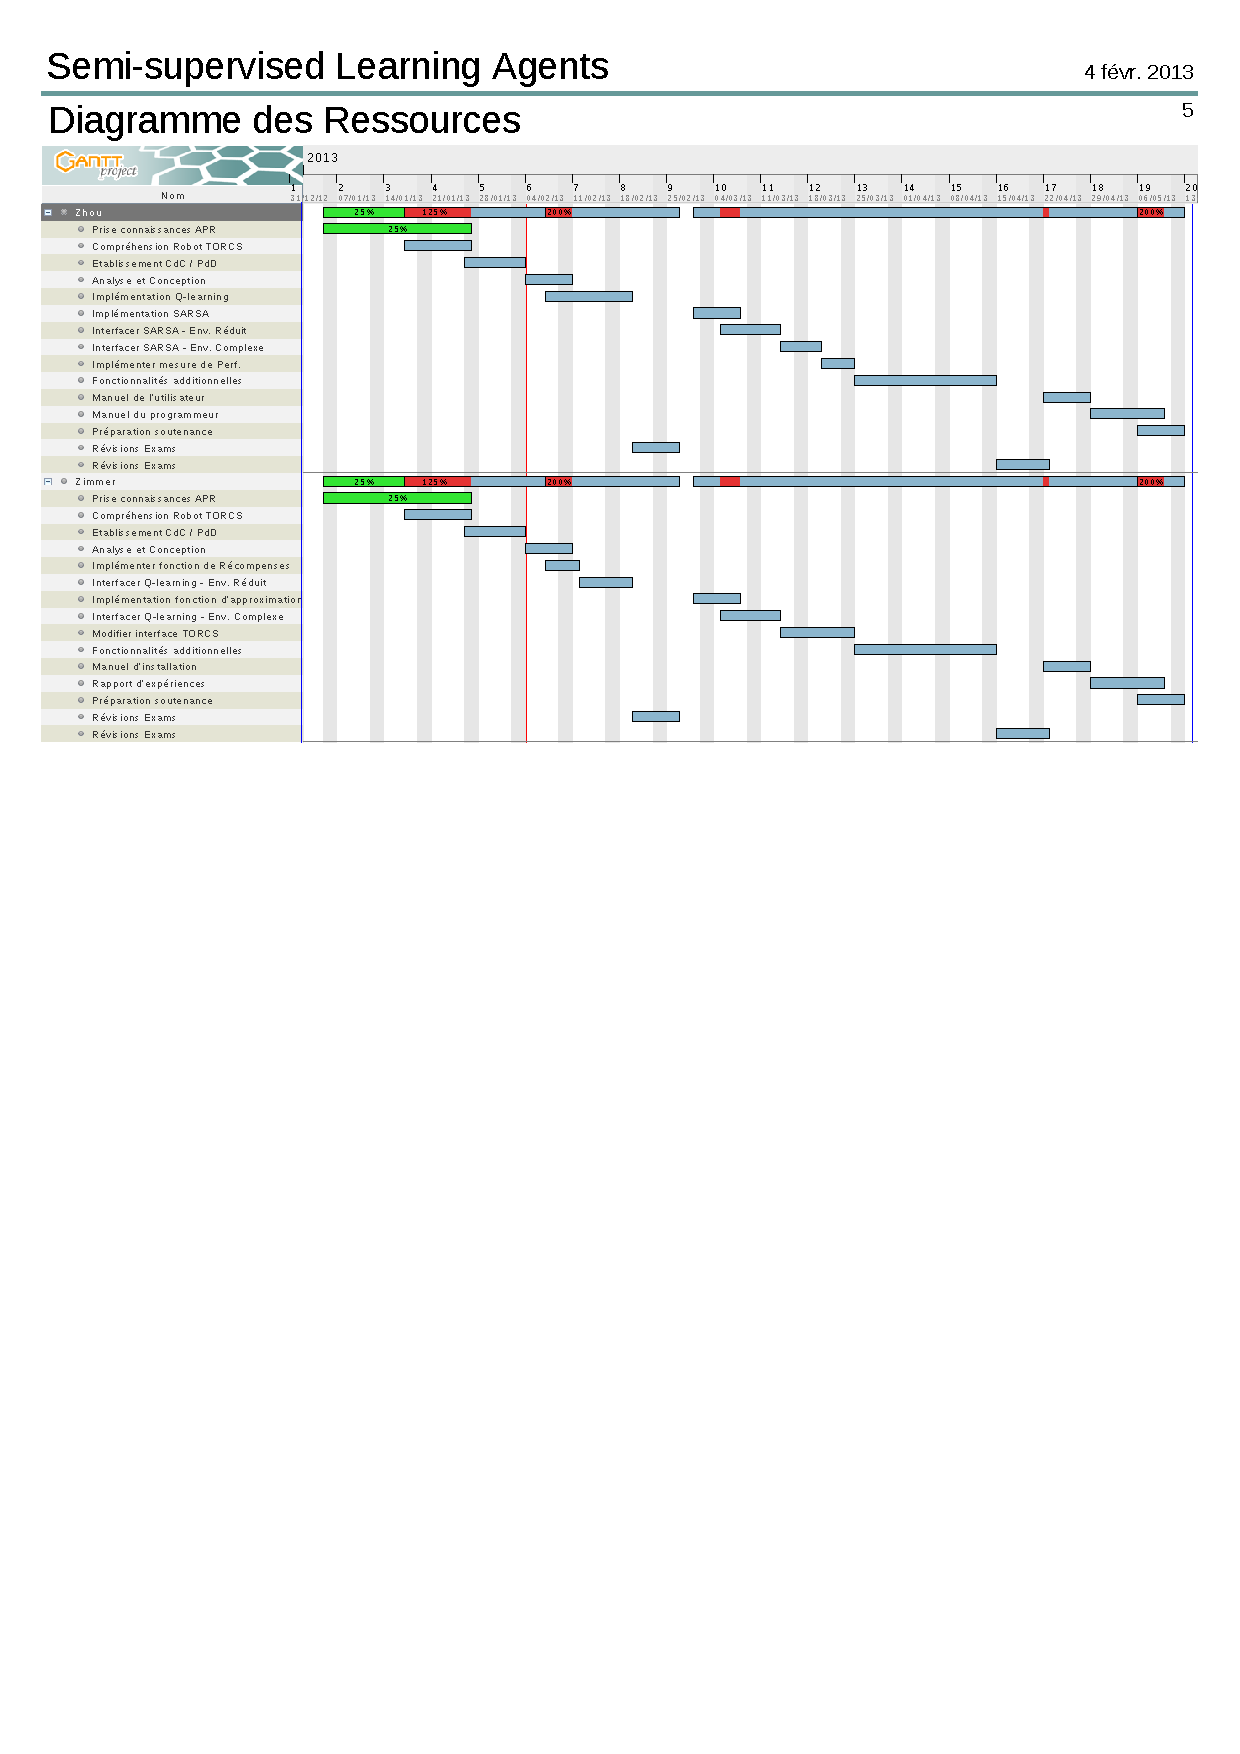
\includegraphics[width=20cm, clip=true, trim= 0 450 0 72]{../images/GanttR.pdf} }
	\caption{Diagramme de Gantt par Ressource \scriptsize{(zoomer pour meilleur qualité)}}
      \end{figure}
	
      \begin{figure}[h!]
	\centerline{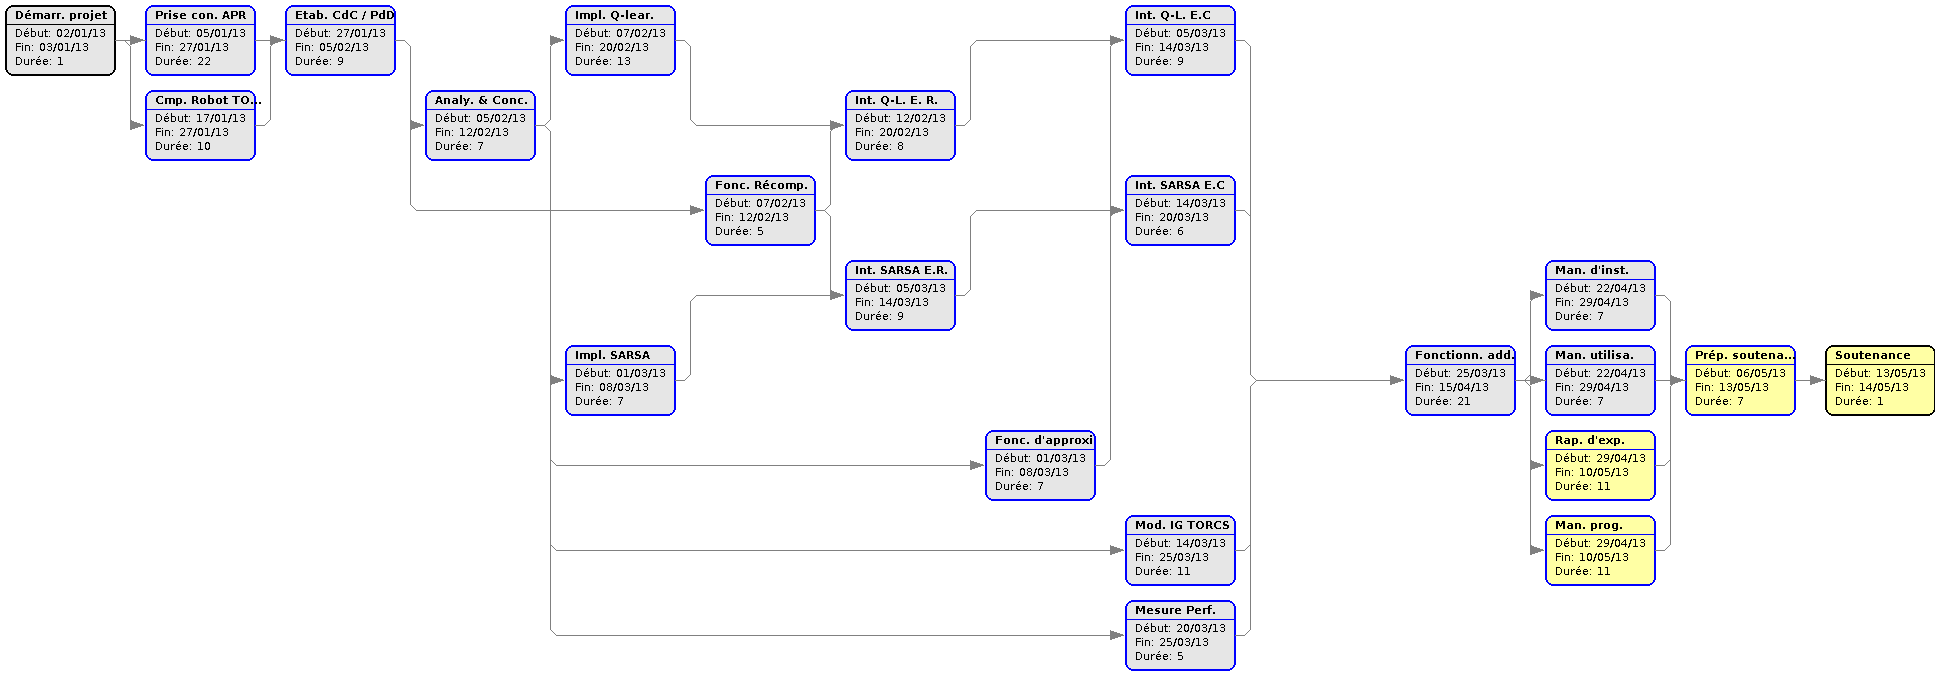
\includegraphics[width=19cm, clip=true, trim= 0 0 0 0]{../images/Gantt_PERT.png} }
	\caption{Diagramme de PERT \scriptsize{(zoomer pour meilleur qualité)}}
      \end{figure}
	
\begin{center}

\end{center}



\end{document}



